\chapter{Background}                                \label{Chapter:background}

    In this chapter, an introduction is given on the needle-free jet injection and the progress of applying the use of linear direct-drive machines on jet injection, which lead to the definition of the research goal of this thesis. Then this chapter further provided electromagnetic field theory, available motors modeling techniques and optimization approaches to realize the methods later discussed in this thesis.


% ===================================================================================================
% === NEW SECTION === NEW SECTION === NEW SECTION === NEW SECTION === NEW SECTION === NEW SECTION ===
% ===================================================================================================
\section{Transdermal drug delivery}                 \label{Chapter:background/transdermal drug delivery}
    % \subsection{Problems}                           \label{Chapter:background/transdermal drug delivery/problems}
    % \subsection{Alternative methods}                \label{Chapter:background/transdermal drug delivery/alternative methods}

    Transdermal drug delivery is a method of delivery for pharmaceutical solutions that are unsuitable for ingestion or cannot penetrate through the skin. Many vaccines and insulin are delivered by this approach\,\cite{sadrzadeh2007}. While being efficient and precise, transdermal drug delivery via hypodermic needle is time-consuming, labour intensive, and hazardous. The procedure requires the operator to attach a hollow needle to a syringe, then extract the drug, eliminate air bubbles in the syringe and sterilize the applied area thoroughly. Once prepared, the operator can slowly inject a high volume of drug. During disposal, needle stick is a safety hazard. Needle-stick injuries hold a high risk of transmitting contagious diseases such as HIV, HBV, and HCV. Percutaneous sharps injuries have affected millions of individuals across the world\,\cite{pruss2005}. 
    
    Today, needle sticks and sharp objects still represent a significant challenge in creating a safe environment for professional health care practitioners. Pain\,\cite{schneider1994} and needle-phobia\,\cite{hamilton2005,Nir2003} are other motivations to develop and popularize alternative strategies.
    
    Some distinct transdermal drug delivery methods were invented to tackle issues of needle injection. They include iontophoresis\,\cite{dhote2012}, sonophoresis\,\cite{bommanan1992}, permeation enhancement by chemicals\,\cite{karande2006}, micro-needles on patches\,\cite{cormier2004}, and jet injection\,\cite{taberner2006}. 

% ===================================================================================================
% === NEW SECTION === NEW SECTION === NEW SECTION === NEW SECTION === NEW SECTION === NEW SECTION ===
% ===================================================================================================
\section{Needle-free Jet Injection}                 \label{Chapter:background/needle-free jet injection}
    
    
    % -----------------------------------------------------------------------------------
    % --- NEW SUB SECTION --- NEW SUB SECTION --- NEW SUB SECTION --- NEW SUB SECTION --- 
    % -----------------------------------------------------------------------------------
    \subsection{How it works}                       \label{Chapter:background/needle-free jet injection/how it works}
    
        \ac{NFJI}, commonly called “hypo-spray” in science fiction, was patented in 1960\,\cite{ismach1962}. Figure\,\ref{fig:chapter/background/explain needle free/original injector} shows the original \acs{NFJI} device, “Ped-O-Jet” in use for the purpose of mass vaccination\,\cite{DictionnairesetEncyclopediessurAcademic}. This device was invented  upon realizing that pressurized fluid can penetrate human skin. Fluid streams of appropriate diameter and velocity can produce sufficient pressure to breach through the skin layers up to a particular desired depth. 
        
        \begin{figure*}[!ht]
            \centering
            \subfloat[Ped-O-Jet in use\,\cite{DictionnairesetEncyclopediessurAcademic}]{
                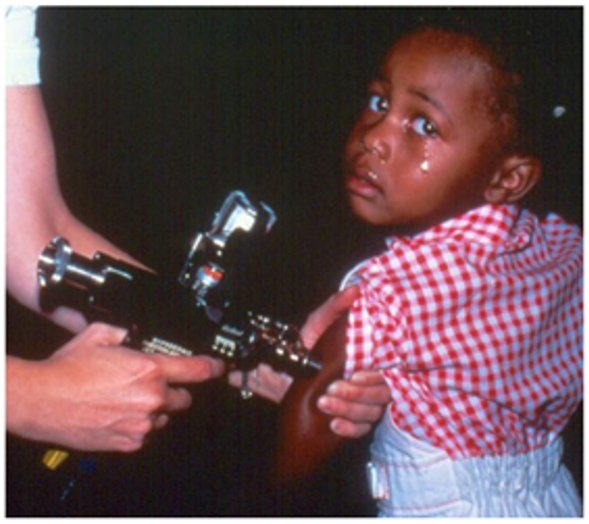
\includegraphics[width=0.35\textwidth]{chap2/images/original_injector.png}
                \label{fig:chapter/background/explain needle free/original injector}
            }
            \qquad
            \subfloat[Needle injection versus Needle-free injection\,\cite{injex2012}]{
                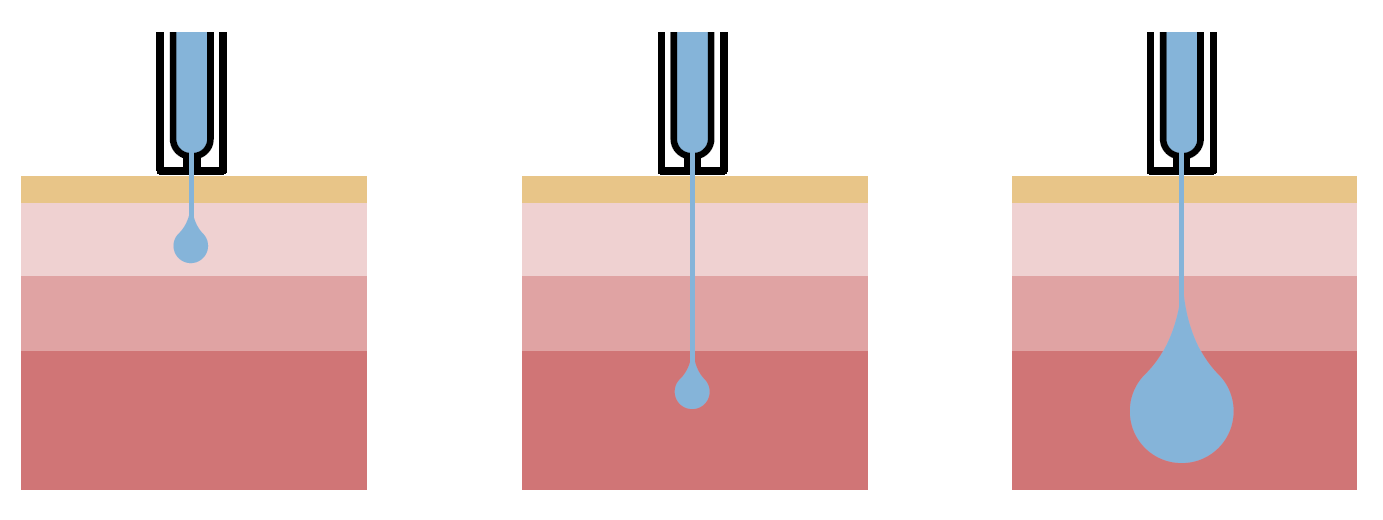
\includegraphics[width=0.5\textwidth]{chap2/images/needle_vs_needle_free.png}
                \label{fig:chapter/background/explain needle free/needle vs no needle}
            }
            \caption{
                Needle-free jet injection's history and concept explained.
            }   \label{fig:chapter/background/explain needle free}
        \end{figure*}
        
        A subcutaneous or intramuscular jet injection could be realized by forcing a fluid jet of $\mathrm{76-360\,\mu m}$  diameter to penetrate the human skin at a speed faster than $\mathrm{100 \,m/s}$\,\cite{mitragotri2006,Hogan2006}. Figure\,\ref{fig:chapter/background/explain needle free/needle vs no needle} shows that an ideal jet injection would deliver the drug in a similar manner to a hypodermic needle injection\,\cite{InsuJet2013}.
        
        % Even though this method adopts the use of needle-free apparatus, biological material can still be unwillingly transferred if there are no appropriate decontamination schemes. Concerns have been raised in the literature about potential transmission of blood-borne infections by multiple-use \acs{NFJI} since the early 1970s\,\cite{kremer1970, weintraub1988}. Figure\,\ref{fig:chapter/background/injection mechanism} illustrates three possible mechanisms of how blood contamination can take place\,\cite{hoffman2001}. 
        
        % \begin{figure*}[!ht]
    
        %     \centering
        %     \subfloat[]{
        %         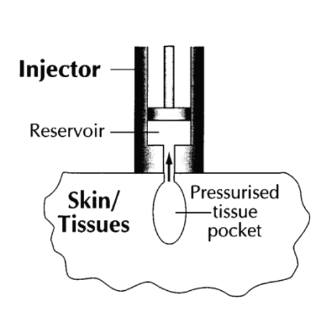
\includegraphics[width=0.29\textwidth]{chap2/images/jet_injection_mechanism_1.png}
        %         \label{fig:chapter/background/injection mechanism/1}
        %     }
        %     \subfloat[]{
        %         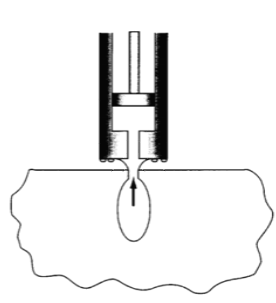
\includegraphics[width=0.25\textwidth]{chap2/images/jet_injection_mechanism_2.png}
        %         \label{fig:chapter/background/injection mechanism/2}
        %     }
        %     \subfloat[]{
        %         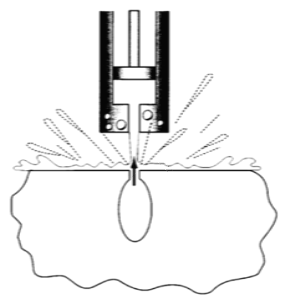
\includegraphics[width=0.27\textwidth]{chap2/images/jet_injection_mechanism_3.png}
        %         \label{fig:chapter/background/injection mechanism/3}
        %     }
        %     \caption{
        %         3 possible mechanisms of blood contamination in ‘mass campaign jet injectors’. 
        %     }   \label{fig:chapter/background/injection mechanism}
        % \end{figure*}    
        
        % Scenario in Figure\,\ref{fig:chapter/background/injection mechanism/1} shows that tissues return fluid into the reservoir as injection pressure diminishes. Liquid flows out to the tip of the injector as the injector’s tip is removed from the applied area as illustrated in Figure\,\ref{fig:chapter/background/injection mechanism/2}. Scenario in Figure\,\ref{fig:chapter/background/injection mechanism/3} displays a ‘splash back’ of jet stream during injection. Uninterrupted, continuous, reuse of \acs{NFJI} has historically caused instances of mass HBV spread\,\cite{canter1990}. For prevention of future mass infection, ‘mass campaign jet injectors’ were disapproved for human use by the World Health Organization\,\cite{who2005}. Nowadays, reusable \acsp{NFJI} for human use must accommodate replaceable syringes. 
    
    
    % -----------------------------------------------------------------------------------
    % --- NEW SUB SECTION --- NEW SUB SECTION --- NEW SUB SECTION --- NEW SUB SECTION --- 
    % -----------------------------------------------------------------------------------
    \subsection{Underlying mechanics}               \label{Chapter:background/needle-free jet injection/underlying mechanics}
    
        \begin{figure*}[!ht]
            \centering
            \subfloat[The general shape of jet penetration into polyacrylamide gel.]{
                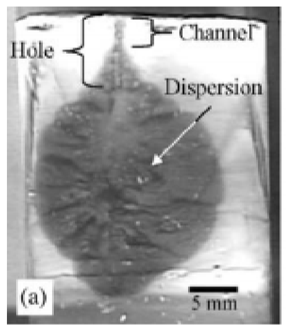
\includegraphics[width=0.28\textwidth]{chap2/images/jet_injection_mechanics_1.png}
                \label{fig:chapter/background/underlying mechanics/1}
            }
            \quad
            \subfloat[Side view of the same gel sample.]{
                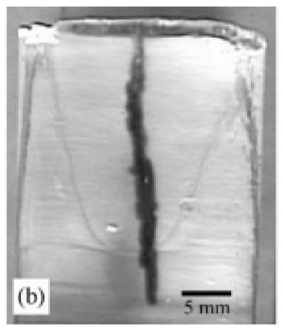
\includegraphics[width=0.28\textwidth]{chap2/images/jet_injection_mechanics_2.png}
                \label{fig:chapter/background/underlying mechanics/2}
            }
            \quad
            \subfloat[The transverse slice of the gel shows the presence of the cylindrical channel.]{
                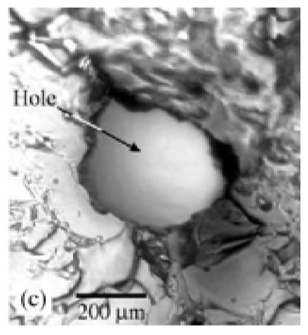
\includegraphics[width=0.3\textwidth]{chap2/images/jet_injection_mechanics_3.png}
                \label{fig:chapter/background/underlying mechanics/3}
            }
            \caption[Needle-free injection into a polyacrylamide gel containing $20\%$ acrylamide]{
                Needle-free injection into a polyacrylamide gel containing $20\%$ acrylamide\,\cite{schramm2004}.
            }   \label{fig:chapter/background/underlying mechanics}
        \end{figure*}
    
        To explore the mechanics of NFJI into the skin, an experiment was conducted where a high-speed camera monitored a spring-driven jet injection into polyacrylamide gel as a test bed\,\cite{Schramm-Baxter2004b} as shown in Figure\,\ref{fig:chapter/background/underlying mechanics}. Motion analysis demonstrated the presence of three distinct jet injection phases: erosion, stagnation, and dispersion. The erosion phase is the period when the jet penetrates in the form of a cylindrical channel. The brief reduction of upfront kinetic energy causes the fluid to start building up at a certain depth, described as the stagnation phase. The dispersion phase is where a drug volume infiltrates the cracks propagated within the gel by fluid pressure during previous phases. The maximum depth was controlled by altering the jet velocity at erosion, and likewise, the amount of drug delivered is determined by the jet speed at the dispersion phase\,\cite{Stachowiak2009}.
        
        
        \begin{figure*}[!ht]
            \centering
            \subfloat[]{
                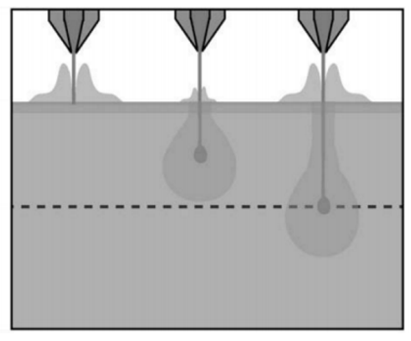
\includegraphics[width=0.515\textwidth]{chap2/images/1_speed_injection.png}
                \label{fig:chapter/background/2 speeds mechanics/just 1 speed}
            }
            \qquad
            \subfloat[]{
                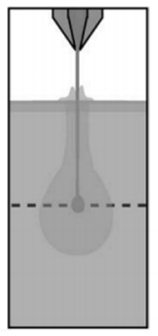
\includegraphics[width=0.20\textwidth]{chap2/images/2_sppeds_injection.png}
                \label{fig:chapter/background/2 speeds mechanics/2 speeds}
            }
            \caption[Need for temporal control of jet velocity in needle-free transdermal drug delivery: (a) constant low-velocity delivery (left), medium-velocity delivery (centre), and high-velocity delivery (right); (b)Desired drug delivery showing sufficient penetration depth and minimal pooling. Dotted line represents the desired depth of injection.]{
                Need for temporal control of jet velocity in needle-free transdermal drug delivery\,\cite{Mitragotri2005}: (a) constant low-velocity delivery (left), medium-velocity delivery (centre), and high-velocity delivery (right); (b)Desired drug delivery showing sufficient penetration depth and minimal pooling. Dotted line represents the desired depth of injection.
            }   \label{fig:chapter/background/2 speeds mechanics}
        \end{figure*}
        
        
        Difficulty in controlling depth injection and ‘splash back’ were the result of using a single jet velocity\,\cite{schramm2002}. Figure\,\ref{fig:chapter/background/2 speeds mechanics/just 1 speed} explains the need for temporal control of the jet velocity in needle-free transdermal drug delivery\,\cite{Mitragotri2005}. At constant low pressure, the jet may not penetrate into the skin (left), while constant, medium-pressure jet velocity may breach the skin with minimal ‘splash back’ yet reach an insufficient depth (middle). A high-pressure stream may reach the desired depth, but fluid pooling cannot be avoided (right). With the use of an initial high jet pressure followed by a lower holding pressure, it was predicted that ’splash back’ would be reduced while the jet disperses at the correct depth\,\cite{wendell2006}. This concept is portrayed in Figure\,\ref{fig:chapter/background/2 speeds mechanics/2 speeds} and \ref{fig:chapter/background/2 speeds ideas}. Taberner et al.\,\cite{taberner2012} demonstrated that the use of a high degree of fluid stream velocity control can deploy this strategy reliably.
        
        
        \begin{figure}[h]
            \centering
            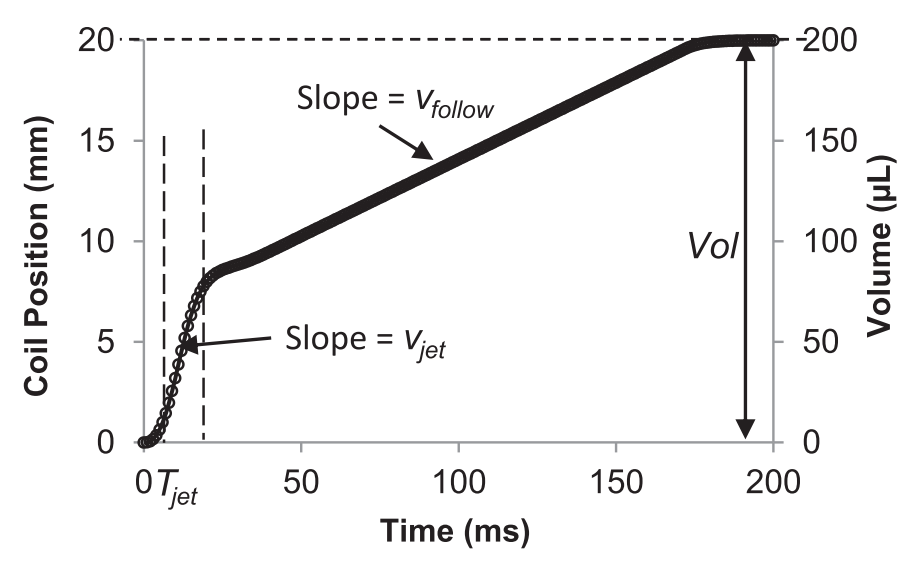
\includegraphics[width=0.75\textwidth]{chap2/images/2_jet_speeds_idea.png}
            \caption[A typical 2 speeds jet injection trajectory; $v_{jet}=200\,\mathrm{m/s}$ to reach the desired injection depth and $v_{follow}=20\,\mathrm{m/s}$ to reduce ‘splash back’]{A typical 2 speeds jet injection trajectory; $v_{jet}=200\,\mathrm{m/s}$ to reach the desired injection depth and $v_{follow}=20\,\mathrm{m/s}$ to reduce ‘splash back’ \,\cite{taberner2012}}
          \label{fig:chapter/background/2 speeds ideas}
        \end{figure}
    
    
    % -----------------------------------------------------------------------------------
    % --- NEW SUB SECTION --- NEW SUB SECTION --- NEW SUB SECTION --- NEW SUB SECTION --- 
    % -----------------------------------------------------------------------------------
    \subsection{Commercially available options}     \label{Chapter:background/needle-free jet injection/commercially available options}
        
        Commercially available \acsp{NFJI} including BIOJECT Zeajet\footnote{http://www.bioject.com/products/zetajet-info} , INJEX 30\footnote{https://www.injex.com.au/injex/injex} , PHARMAJET Stratis\footnote{http://pharmajet.com/fda-approved-needleless-flu-shot} , COMFORT-IN\footnote{http://www.comfort-in.com/diabetes.html}  are spring-powered, small, portable, handheld devices. They are capable of delivering either vaccination or insulin in a small dose, with volume limited to $\mathrm{300\,\mu L}$. Figure\,\ref{fig:chapter/background/pharma jet stratis} illustrates the appearance, construction, and mechanism of the spring-loaded PHARMAJET Stratis NFJI as an example. These devices come in various shapes, sizes, injection volumes, and target skin layers. Their primary structure consists of three main components:
        \begin{itemize}
            \item Energy storage - compressed gas, spring coil or explosives\,\cite{taberner2012}, which are often accompanied by a recharging device,
            \item Piston - actuator with various size and triggering method to accomplish desired pressure profile as well as injection volume specification,
            \item Replaceable syringe - single use container with orifice hole diameter of under $\mathrm{1\,mm}$.
        \end{itemize}
        
        \begin{figure*}[!ht]
            \centering
            \subfloat[\acs{NFJI} device and replaceable syringe]{
                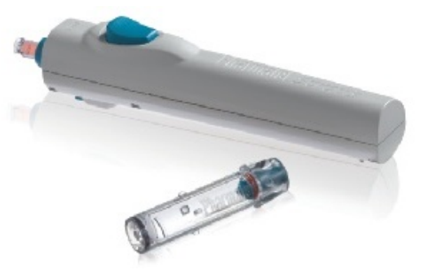
\includegraphics[width=0.40\textwidth]{chap2/images/pharma_jet_stratis.png}
                \label{fig:chapter/background/pharma jet stratis/full view}
            }
            \qquad
            \subfloat[Spring loaded mechanism of the device]{
                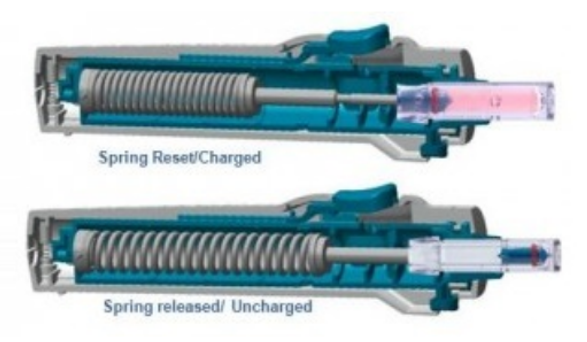
\includegraphics[width=0.45\textwidth]{chap2/images/pharma_jet_stratis_cut_view.png}
                \label{fig:chapter/background/pharma jet stratis/cut view}
            }
            \caption[SUNFJI Pharma Jet Stratis™ from PharmaJet™]{
                SUNFJI Pharma Jet Stratis™ from PharmaJet™\,\cite{PharmaJet2011}
            }   \label{fig:chapter/background/pharma jet stratis}
        \end{figure*}
        
        Once triggered, stored energy produces varying pressure on the injection cylinder until the piston reaches the end of its track. Different devices utilize different recoil or trigger mechanisms, but no system is capable of monitoring and measuring injection performance. Instead of concentrated fluid delivery in a narrow stream down the tissue, these devices tend to spread the drug content in a cone shape\,\cite{baxtex2005}. Figure\,\ref{fig:chapter/background/jet injection effectiveness/mechanical devices pressure curve} shows the sharp peak and oscillating nature of the pressure produced by the injection stream of a BIOJECT Vitajet 3™ spring powered \acs{NFJI}\,\cite{schramm2002}. Schneider et al.\,\cite{schneider1994} reported that without stroke velocity and position control, the sharp fluid pressure profile peak could cause pain, bruises, bleeding, and blisters. Their studies also showed evidence that the same spring powered NFJI device exhibits inconsistent performance across different skin types and conditions. 
        
        Despite being a safer alternative, mechanically powered \acsp{NFJI} require manual recharging. Thus, the average cycle time was recorded to be no faster than that of a conventional hypodermic needle injection\,\cite{PharmaJet2011}. More advanced \acsp{NFJI} like LECTRAJET  have shown the capability of automatic spring recoil to reduce reload time. Lack of pressure control, low injection volume (typically $0.05$ to $0.3\,\mathrm{mL}$), long cycle time, poor repeatability and reproducibility are drawbacks of commercially available mechanically powered \acsp{NFJI}.
        
        \begin{figure*}[!ht]
            \centering
            \subfloat[Typical pressure curve for a $152\,\mathrm{\mu m}$ diameter nozzle from injector Vitajet\,3™]{
                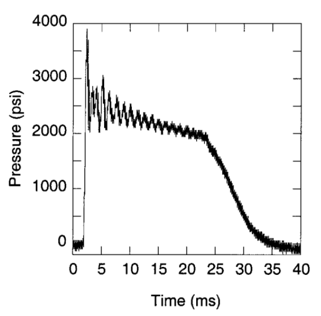
\includegraphics[width=0.43\textwidth]{chap2/images/jet_injection_pressure_curve.png}
                \label{fig:chapter/background/jet injection effectiveness/mechanical devices pressure curve}
            }
            \qquad
            \subfloat[Delivery of mannitol by jet injection into human (A), porcine abdominal (B), and porcine dorsal skin (C) using the same device at $177\,\mathrm{m/s}$. There is a significant difference between each type of skin tested ($p=0.001$)]{
                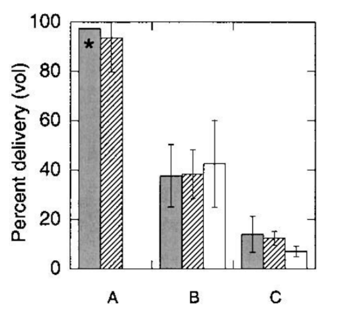
\includegraphics[width=0.45\textwidth]{chap2/images/jet_injection_delivery_study.png}
                \label{fig:chapter/background/jet injection effectiveness/delivery statistic}
            }
            \caption[Results of different jet injection study on mechanically powered \acs{NFJI} devices demonstrating rough pressure profile and poor adaptability.]{
                Results of different jet injection study on mechanically powered \acs{NFJI} devices demonstrating rough pressure profile and poor adaptability\,\cite{schramm2002}.
            }   \label{fig:chapter/background/jet injection effectiveness}
        \end{figure*}


    % -----------------------------------------------------------------------------------
    % --- NEW SUB SECTION --- NEW SUB SECTION --- NEW SUB SECTION --- NEW SUB SECTION --- 
    % -----------------------------------------------------------------------------------
    \subsection{Controllable \acs{NFJI} devices}    \label{Chapter:background/needle-free jet injection/Controllable NFJI}
    
        Recent achievements in high power density actuators have enabled successful prototypes of electronically controlled \acsp{NFJI} which were capable of real-time jet velocity control. A previous study suggests four advantages of electronic control over traditional needle injection and mechanically powered jet injection\,\cite{henmond2013}:
        
        \begin{itemize}
            \item Controllable - capable of maintaining high pressure without the need of trading-off for injection volume,
            \item Reliable - capable of producing consistent jet pressure on a broad range of skin properties and different injection types,
            \item Versatile - automatic reload under closed loop control or injection volume control,
            \item Measurable - convenient in monitoring progress to evaluate the performance of injection.
        \end{itemize}
        
        This class of device performs injections by utilizing different electrically powered actuators: dynamically controlled piezo-electric actuators\,\cite{Stachowiak2009}, laser pulsed microjets\,\cite{tawaga2013, park2012} and Lorentz force voice coil motors\,\cite{taberner2006,hemond2006}. Piezo-electric and laser pulse methods are limited to sub $\mathrm{\mu L}$ injections. Scaling of Piezo-electric technology to hundreds of $\mathrm{mL}$ range in injection volume simply appears ambitious. Cumbersome ‘off-the-shelf’ voice coil actuators which will be explored in \ref{Chapter:background/voice coil motors for NFJI} are not yet suitable to become handheld. Recently, Zhang et al. has shown a \acs{NFJI} device powered by commercial rotary motor and specialized differential screw structure, capable of delivering $10\,\mathrm{mL}$ with the input power of $450\,\mathrm{W}$. Although the concept of utilizing synchronous rotary motor for \acs{NFJI} was proven, the volume delivered that a similar system could achieve will be unlikely to reach $1000\,\mathrm{mL}$.

% ===================================================================================================
% === NEW SECTION === NEW SECTION === NEW SECTION === NEW SECTION === NEW SECTION === NEW SECTION ===
% ===================================================================================================
\section{Voice coil motors for \acs{NFJI}}          \label{Chapter:background/voice coil motors for NFJI}
    
    
    % -----------------------------------------------------------------------------------
    % --- NEW SUB SECTION --- NEW SUB SECTION --- NEW SUB SECTION --- NEW SUB SECTION --- 
    % -----------------------------------------------------------------------------------
    \subsection{Principle of operation}             \label{Chapter:background/voice coil motors for NFJI/principle}


    The \ac{VCM} is a type of Lorentz-force actuator. \acsp{VCM} can either have the magnet or the coil as a moving part. Figure\,\ref{fig:chapter/background/vcm cut view} presents the construction of a moving coil configuration\,\cite{taberner2006}. Here, a Nd-Fe-B magnet is used to generate the magnetic field. The magnet is placed between a steel top plate and the steel casing to direct the flow of magnetic flux in a contained loop. In between the top plate and steel case is a region of air gap that allows the copper winding to slide up or down. A directional force $F$ is proportional to the strength of the magnetic field $B$ through the wire, and the electric current per unit area $J$ passing through the coil:
    
    
    \begin{equation}
        \overrightarrow{F}=\overrightarrow{J}\times \overrightarrow{B}
        \label{eq:force produce via field and current}
    \end{equation}

    The polarity of the current also dictates which direction the coil will move. It is clear that more force can be generated by either strengthening the magnetic field or increasing the current through the coil. Adjusting other parameters such as coil geometry, coil thickness, magnet materials, and aspect ratio can alter the motor force constant and stroke length.
    
    
    \begin{figure}[!ht]
      \centering
      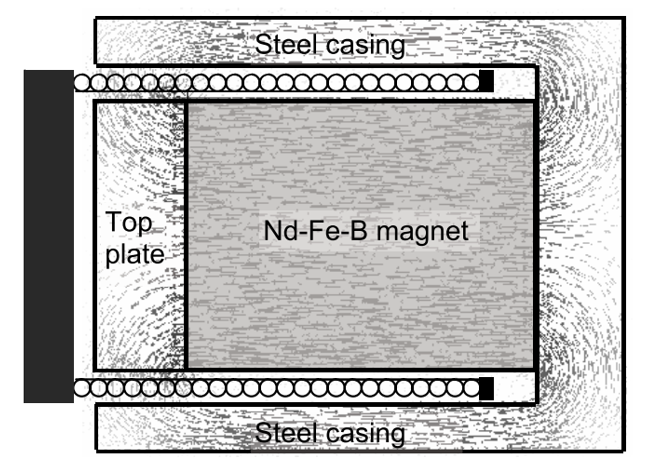
\includegraphics[width=0.5\textwidth]{chap2/images/vcm_cut_view.png}
      \caption[Construction of a voice coil motor with moving coil]{Construction of a voice coil motor with moving coil\,\cite{taberner2006}.}
      \label{fig:chapter/background/vcm cut view}
    \end{figure}
    
    
    % -----------------------------------------------------------------------------------
    % --- NEW SUB SECTION --- NEW SUB SECTION --- NEW SUB SECTION --- NEW SUB SECTION --- 
    % -----------------------------------------------------------------------------------
    \subsection{Application to \acs{NFJI}}          \label{Chapter:background/voice coil motors for NFJI/application}
    
    
    Recently, collaboration between the \ac{MIT} and \ac{ABI} Bioinstrumentation Labs has created two prototype jet injectors actuated by a customized Lorentz-force \ac{VCM}\,\cite{taberner2006,ruddy2014} shown in Figure\,\ref{fig:chapter/background/vcm injectors}. With the use of real-time feedback control, these systems have demonstrated highly controllable and repeatable injections against a broad range of different test tissues, depths, and dosage volumes\,\cite{taberner2012}. With the successful prototypes, the vision was to advance the prototypes into portable and high volume injector devices.


    \begin{figure*}[!ht]
        \centering
        \subfloat[]{
            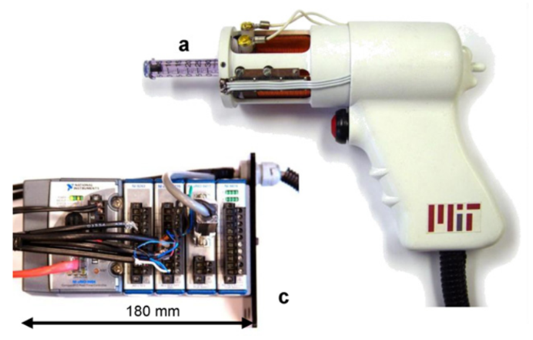
\includegraphics[width=0.5\textwidth]{chap2/images/vcm_taberner2006.png}
            \label{fig:chapter/background/vcm injectors/taberner2006}
        }
        \qquad
        \subfloat[]{
            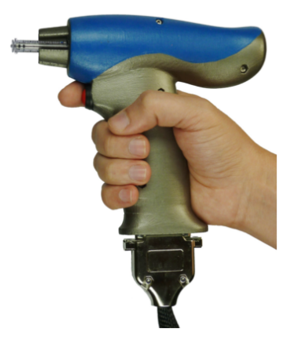
\includegraphics[width=0.28\textwidth]{chap2/images/vcm_ruddy2014.png}
            \label{fig:chapter/background/vcm injectors/ruddy2014}
        }
        \caption[Lorentz-force \acs{VCM} actuated \ac{NFJI}: Handheld injector and cRIO controller system (a)\,\cite{taberner2006}; Hand-held injector and charged capacitor amplifier/controller system (b).]{
            Lorentz-force \acs{VCM} actuated \ac{NFJI}: Handheld injector and cRIO controller system (a)\,\cite{taberner2006}; Hand-held injector and charged capacitor amplifier/controller system (b)\,\cite{ruddy2014}.
        }   \label{fig:chapter/background/vcm injectors}
    \end{figure*}
    
    
    \begin{figure}[!ht]
      \centering
      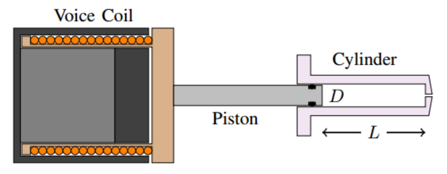
\includegraphics[width=0.5\textwidth]{chap2/images/vcm_for_nfji.png}
      \caption[A basic schematic of a voice coil actuated \acs{NFJI}. $L$ and $D$ are the cylinder’s working length (stroke length) and diameter, respectively.]{A basic schematic of a voice coil actuated \acs{NFJI}. $L$ and $D$ are the cylinder’s working length (stroke length) and diameter, respectively\,\cite{ruddy2014}.}
      \label{fig:chapter/background/vcm for nfji}
    \end{figure}
    
    
    Figure\,\ref{fig:chapter/background/vcm for nfji} shows a basic schematic of a voice coil actuated \acs{NFJI}. $L$ and $D$ are the cylinder’s working length (stroke length) and diameter, respectively\,\cite{ruddy2014}. In this device, injection volume can be enlarged by either up-scaling the ampoule diameter $D$, or the working stroke length $L$, or both. A jet injector with an ampoule diameter $D$ requires an actuation force $F$ to be provided by the motor. For constant peak jet velocity $v_{jet}$ and fluid density $\rho$:
    
    
    \begin{equation}
        F=\frac{\pi}{8}\rho {v_{jet}}^2 D^2
        \label{eq:force produce relationship in motor powered NFJI}
    \end{equation}
    
    
    If syringe’s diameter\,$D$ is chosen to scale with injection volume, electric power\,$P$ needs to scale with the square of $D$’s scaling ratio due to the relationship:
    
    
    \begin{equation}
        P=F v_{piston}
        \label{eq:power required for F and v_piston}
    \end{equation}
    
    
    where $v_{piston}$ is the speed of the moving piston. If the syringe’s diameter  is chosen to scale with the injection volume, the electric power\,$P$ needs to scale with the square of $D$’s scaling ratio. Given that the jet velocity follows the varying velocity strategy explained in Section\,\ref{Chapter:background/needle-free jet injection/underlying mechanics}, the motor needs to achieve the peak jet velocity required for the brief erosion phase, then the lower jet velocity speed for the dispersion phase. For only for a very short period, the device is required to produce much more power than its average power drawn. It is not common to find energy storage and powering devices at power magnitude of many kilowatts, provided in a portable fashion.
    
    
    % -----------------------------------------------------------------------------------
    % --- NEW SUB SECTION --- NEW SUB SECTION --- NEW SUB SECTION --- NEW SUB SECTION --- 
    % -----------------------------------------------------------------------------------
    \subsection{Scaling properties and limitations} \label{Chapter:background/voice coil motors for NFJI/scaling and limitation}
    
    
    The following key relationship relates the power dissipation on the motor winding $P$, density of fluid to be delivered $\rho$, ampoule volume $V$, jet velocity $v_{jet}$, motor constant $K_m$, and distance travelled by the piston stroke $L$ \cite{Williams2012}:
    
    
    \begin{equation}
        P=\frac{\rho^2 V^2 {v_{jet}}^4}{4 {K_m}^2 L^2}
        \label{eq:power required for F,V,v_jet,K_m, and L}
    \end{equation}
    
    
    To compare the force exerted over the power consumed in different motors, the motor constant $K_m$ measured in $\mathrm{N/\sqrt{W}}$  is typically used. Note that this relationship is true of all direct drive linear motors, which apply force directly to a single injection ampoule without any mechanical coupling transmission.
    
    
    Utilizing a general scaling magnetic and thermal model made for steady-state force production of \ac{PMLSM}\,\cite{Ruddy2011}, an optimal \acs{VCM} hand-piece was built to deliver $\mathrm{300\,\mu L}$ of the drug over a $\mathrm{50\,ms}$ period\,\cite{taberner2006}. The peak power required for this procedure was as high as 10 kW to produce a peak force of $\mathrm{300\,N}$ of over the stroke length of $\mathrm{35\,mm}$. Due to the extremely short duration of the force profile, the heat generated is far from enough to cause permanent demagnetization in the permanent magnet array; thus, the motor design neglects heat transfer. In the same body of work, the authors pointed out that scaling laws of the voice coil actuator fit for needle free injection means that the power $P$ required and motor mass $M$ both grow faster than the injection volume $V$:
    
    
    \begin{equation}
        M \propto V^{6/5}
        \label{eq:scaling property of VCM}
    \end{equation}


    While the potential of using \acsp{VCM} in portable \acs{NFJI} devices has been proven, this type of motor is power inefficient. Without breakthrough improvements, \acsp{VCM} pose a considerable restriction on the portability of the electronic control system, as well as the size of the injector handpiece motor. Based on the model presented in that work, a \acs{VCM} with mass of over $\mathrm{1\,kg}$ is required to deliver $\mathrm{1\,mL}$. Thus, it was impractical to use a direct-drive linear \acs{VCM} to deliver regular livestock injections, where the volume can be as high to $\mathrm{10\,mL}$. 

% ===================================================================================================
% === NEW SECTION === NEW SECTION === NEW SECTION === NEW SECTION === NEW SECTION === NEW SECTION ===
% ===================================================================================================
\section{Linear synchronous motors for NFJI}        \label{Chapter:background/linear synchronous motors for NFJI}

    
    \acp{LSDDM} are actuators that can drive a motion load without an intermediate mechanism such as gears, screws or crank shafts\,\cite{JacekF.GierasZbigniewJ.Piech2017}. The absence of auxiliary mechanical adaptation increases their reliability. In high speed applications, linear direct-drive synchronous motors can have higher efficiency and a higher dynamic performance compared to their rotary counter parts. ‘Synchronous’ in the context of electric machines means that the speed of motion is the same as the speed of the travelling magnetic field. The thrust is generated by either the interaction between the traveling magnetic field produced by the poly-phase winding or switched DC windings in an array of magnetic excitation components. 
    
    \acsp{LSDDM} are being used increasingly in applications as varied as automated manufacturing\,\cite{Meessen2010}, transportation\,\cite{Gysen2011,Cao2012,WenxiangZhao2012}, and power generation\,\cite{Li2011,Baker2019}. Although \acsp{LSDDM} have existed for a long time\,\cite{Boldea1997}, to the best of the author’s knowledge, no report has demonstrated that this class of motor can achieve \acs{NFJI} tasks, where a high pulse of force is required from a near stall condition. Technically speaking, a \acs{VCM} is a type of \acs{LSDDM} where there is a single-phase winding driven by a direct current and an array of magnetic excitation with length equal one pole period. True linear synchronous motors, powered by alternating current, provide efficient energy to motion conversion, high force density and excellent capability for precise motion control\,\cite{Trumper1994,Levi1973,Budig2000}.
    
    
    % -----------------------------------------------------------------------------------
    % --- NEW SUB SECTION --- NEW SUB SECTION --- NEW SUB SECTION --- NEW SUB SECTION --- 
    % -----------------------------------------------------------------------------------
    \subsection{Classification}                     \label{Chapter:background/linear synchronous motors for NFJI/classification}
    
        
        The most basic motor consists of two principal components\,\cite{JacekF.GierasZbigniewJ.Piech2017}: the part that produces the travelling magnetic field via a poly-phased copper winding is the armature, and the part that produces magnetic flux or variable reluctance is known as the field excitation system (e.g., a permanent magnet or magnetic field created by induction). \acsp{LSDDM} can come in many different topologies\,\cite{Laithwaite1970}:
        
        
        \begin{itemize}
            \item Moving or fixed armature
            \item Flat (planar) or tubular (cylindrical)
            \item Ferromagnetic core or air core
            \item Slotted or slot-less core (if using back iron core)
            \item Permanent magnet excitation or electromagnetic excitation
            \item Longitudinal flux or transversal/transverse flux
            \item Singly salient or doubly salient
        \end{itemize}
        
        
        Moving or fixed armature simply refers to which part of the motor moves, be it the part containing the armature or part that contain the field excitation system. A moving armature system requires more materials for the fixed field excitation system, which often increases the demand for costly rare-earth permanent magnets. In contrast, the a moving field excitation system often leads to more demanding electronics to control more armature phases. The moving armature configuration is more commonly seen in linear direct drive motors. 
        
        
        The tubular motor concept can be realized by rolling a flat linear machine about its longitudinal axis. Tubular permanent-magnet machines offer the highest efficiency and power over force density and have excellent servo characteristics\,\cite{Eastham1990}. The advantages that the tubular structure can offer over the flat structure includes introducing even magnetic field distribution, reducing wasted winding, and easing the modelling step. Despite superior performance, tubular machines are only more popular than flat machines in research because they are more difficult to manufacture at scale.
        
        
        The ferromagnetic core, whether it is a magnet core or an iron core, exists to provide a low magnetic resistance path between the excitation source and the armature. The subset of \ac{PM} synchronous motors with the use of an iron core has to deal with cogging force. This force stands for the mutual attraction between the PM and iron in the armature. Cogging force is undesirable because it can contribute to a reduction in axial force, vibration and deteriorating control characteristics at low speed\,\cite{Jung1999}. The slotted iron core causes the cogging ripples while the limited iron length causes end effect cogging\,\cite{Lim2002}. Cogging force can be reduced by PM width adjustment\,\cite{Bianchi2002}, asymmetric PM arrangement\,\cite{Chung2016,Bianchi2003a,Cai2012}, a semi-closed slot for the iron core\,\cite{Zhu1997,Bai2015,Zhu2008}, and optimizing iron core geometry\,\cite{Inoue2000,Zhu1997,Wu2008,Zhu2009conf,Zhang2013,Kim2016,Lee2014}. It is better to improve the cogging force profile using mechanical design than to rely on complex control mechanism\,\cite{Jahn1996}. 
        
        
        Recently, the number of research on actuators using permanent magnets has increased significantly. This is due to the availability of high energy rare earth permanent magnet materials from which compact actuators with a high efficiency can be realized. As the size approaches the form factor required for power application such as electric vehicle or energy generation, the difference in performance of induction and permanent magnet machines is small\,\cite{WoosukSung2012Energy-EfficientVehicles,2014Almeida,Chau2008OverviewVehicles,deSantiago2012ElectricalReview}. However, in small form factor use-cases, permanent magnet machines have been reported to outperform induction machines\,\cite{Zhu2007ElectricalVehicles,Yang2015ComparativeApplications}. 
        
        
        The most important distinction for motors perhaps lies in the arrangement of the flux path. Longitudinal flux means that the magnetic field lines are parallel to the direction of motion. Transverse flux, on the other hand, means that the magnetic field lines are perpendicular to the direction of the motion\,\cite{Laithwaite1975}. Further definition of \acfp{LTFM} includes having three-dimensional magnetic flux flow, and there is no coupling between the individual armature and secondary phases. \acsp{LTFM} are especially suitable for low speed and high thrust applications\,\cite{Zhao2015,Shin2015}. This topology allows for containing a large number of poles without compromising the space available for the windings\,\cite{Laithwaite1971}. The structure of this type of motor results in a complex, coupled magnetic and electric circuit. An increase in the number of poles is roughly proportional to the increase in force density. A transversal flux motor, in both rotary and linear forms, can achieve very high work output\,\cite{Ueda2014,Hsu2011,Wang2016,Arshad2001,Siatkowski2008}. Longitudinal flux machines may have discrete structural poles, but for transversal flux machines, discretization of the poles is compulsory\,\cite{Baoming2009}. This structure offers easier and cheaper design, manufacturing and maintenance. However, the segmented core construction and widely open conductor loop lead to high leakage flux, high winding inductance, and low power factor\,\cite{Harris1997,Lu2003}. The iron core takes significantly more volume and weight in transversal flux motors, thus, eddy losses and nonlinear permeability effects must be included to model this type of motor accurately.
        
        
        Both transverse flux motors, or longitudinal flux when called alone, refers to motors that have the flux source (\acs{PM} for instance) separated from the current source, and both sources will not move at the same time as the motor operates. Since the flux source interacts with the current source through an air gap without hard mechanical coupling, we refer to those motors as singly salient motors. On the other hand, doubly-salient motors have "teeth" on both the primary and secondary, resulting in both sides contributing to variation in flux linkage/inductance with position. Belonging  to  the  the  family of doubly-salient permanent magnet motors \,\cite{Cheng2011}, \acp{LFSM} have high  thrust  density, high  tolerance  to  current  overload, lower use  of  permanent  magnet  material,  and  a generally robust construction. They use a passive secondary that can be made out of steel laminations or \ac{SMC} material to reduce eddy current loss to a minimum. Being  able  to ignore eddy currents will play an important role in improving the efficiency of design simulation. The amount of \acs{PM} in a \acs{LFSM} in long stroke applications can be significantly less than that used by a \acs{PMLSM}\,\cite{Aleksandrov2018}. All these advantages are important in bringing a  prototype into manufacturing at scale to reach high reliability. In hindsight, air is a very poor magnetic conductor, thus machines like \acsp{LFSM} with very small flux path resistance should vastly improve motors output. However, since the \acs{LFSM} is still a relatively unexplored topology, the literature has opposing opinions about whether \acsp{LFSM} outperform \acsp{PMLSM}\,\cite{Aleksandrov2018,Wang2008}.
        
        
        One of the disadvantages of synchronous motors is that once the motion and rotating magnetic fields were out synchronism, the motors would not move. A way to work around this problem is to incorporate absolute position sensors or Hall sensors into the control algorithm of the motor. In some cases where the armature requires a large starting torque, the motor is inherently unable to start itself. Even with the help of methods to speed up to synchronism, the armature can always lag if the power supplied is insufficient to cope with the load.
        
        
        Compared to \acsp{VCM}, \acsp{PMLSM} and \acsp{LFSM} in general require far less power to operate. Thus, the same portable power supply built for powering \acsp{VCM} is also capable of driving the other \acsp{PMLSM} and \acsp{LFSM}, provided the technology used has room to expand for multiphase control.
        
        
    % -----------------------------------------------------------------------------------
    % --- NEW SUB SECTION --- NEW SUB SECTION --- NEW SUB SECTION --- NEW SUB SECTION --- 
    % -----------------------------------------------------------------------------------
    \subsection{Summary}                         \label{Chapter:background/linear synchronous motors for NFJI/summary}
        
        
        Previous work at the ABI also conceived a design of a \ac{PMLSM} optimized for \acs{NFJI} application\,\cite{Ruddy2015}. The motor described in that work is a moving armature, tubular, single-sided, back iron cored, slot-less, \acs{PM}, and longitudinal flux linear synchronous motor. The optimized tubular \acs{PMLSM} with a stroke length of $\mathrm{200\,mm}$ and an injection volume of $\mathrm{1\,mL}$ promised a drastic reduction in power requirement compared to \acsp{VCM}. The next step from there is to construct a prototype motor and power amplifier and incorporate them into a complete \acs{NFJI} system. Such motor design will need to incorporate a creative packaging strategy to maintain the hand-held nature of the \acs{NFJI} device. The challenges of constructing \acs{PMLSM} motors with use of PM also include assembly of a large number of small and mutually attracted parts\,\cite{Hwang2012,Shin2012}.
        
        
        While the scaling law of longitudinal flux \acs{PMLSM} requires the stroke length to be long to make a drastic improvement in power efficiency\,\cite{Laithwaite1970}, that is not the case in transversal flux motors. The implication is that the uses of long \acs{NFJI} ampoule strokes and cumbersome packaging mechanism can be avoided altogether if we decided to adopt linear transversal flux motors. The use of newer types of motor such as \acsp{LFSM} should also be explored because it is possible to save a significant amount of rare-earth permanent magnet and have near equivalent performance to \acs{PMLSM}.


% ===================================================================================================
% === NEW SECTION === NEW SECTION === NEW SECTION === NEW SECTION === NEW SECTION === NEW SECTION ===
% ===================================================================================================
\section{Electromagnetic field theory}              \label{Chapter:background/electromagnetic field theory}


    The emergence of energy convergence of energy conversion applications and modern electronics have led to a large variety of magnetic materials supplied in all shapes and size. The phenomenon of a material forming a permanent magnet or temporary microscopic dipoles under the influence of a magnetic field is known as ferromagnetism. While all materials are magnetic to some extent, only ferromagnetic materials can form strong magnetic flux density $B$ under the influence of an external magnetizing field $H$. In this body of work, they are referred as ‘$B$-field’ and ‘$H$-field’. 
    

    % -----------------------------------------------------------------------------------
    % --- NEW SUB SECTION --- NEW SUB SECTION --- NEW SUB SECTION --- NEW SUB SECTION --- 
    % -----------------------------------------------------------------------------------
    \subsection{Quasi-static Maxwell's equations}     \label{Chapter:background/electromagnetic field theory/quasi-static maxwell equations}
    
    
        Maxwell's equations describe how electric and magnetic fields are generated by charges, current, and the changes in either magnetic or electric fields. As a set of \acp{PDE}, they provide a foundation for understanding classical electromagnetism, optics and even electrical circuits. In the case of motors, the electromagnetic fields travel drastically slower than the maximum speed possible for electromagnetic waves, known as the speed of light. The time rates of changes of relevant electromagnetic fields are sufficiently low that they can be simplified to the set of quasi-static Maxwell's equations\,\cite{Melcher1981}. The quasi-static Maxwell's equations in differential forms are defined as:
    
    
        \begin{equation}
            \nabla \times H = J_f
            \label{eq:ampere's circuit law}
        \end{equation}
        
        \begin{equation}
            \nabla \cdot B = 0
            \label{eq:gauss's magnetism law}
        \end{equation}
        
        \begin{equation}
            \nabla \times E = \frac{\partial B}{\partial t}
            \label{eq:maxwell-faraday's law}
        \end{equation}
    
        \begin{equation}
            \nabla \cdot D = \rho
            \label{eq:gauss's law}
        \end{equation}
    
    
        where $J_f$ is the free current density in the conductor, $E$ is the electric field, $D$ is the electric flux density and $\rho$ is the free electrical charge destiny. Bold symbols here represent vector quantities. Even existing in a simplified form, these equations are coupled \acsp{PDE}, which are often very difficult to solve analytically. Like any differential equation, boundary conditions and initial conditions are necessary for a unique solution. Numerical methods can be used to approximate the result, but an exact solution is not yet found.
        
        
        The Maxwell's equations can be rewritten to by introducing the magnetic vector potential $A$, free space permeability ${\mu}_0$, and the conductor relative permeability ${\mu}_r$, true for quasi-static conditions:
        
        
        \begin{equation}
            \nabla \times A = B
            \label{eq:curl of A is B}
        \end{equation}        
        
        \begin{equation}
            M = M_0 + M_f
            \label{eq:component of magnetization}
        \end{equation}     
        
        \begin{equation}
            {\nabla}^2 A = -{\mu}_0 ({\mu}_r J_f + \nabla \times M_0)
            \label{eq:relation of A to Magnetization and free current}
        \end{equation}        
        
        
        The magnetization $M$ of a ferromagnetic material has two components. The first magnetization component $M_0$ results from permanent magnetization in hard magnetic material like permanent magnets. The secondary magnetization $M_s$ is related to the magnetic field $H$, which can be temporary:
        
        
        \begin{equation}
            M_s = \chi_m H
            \label{eq:secondary magnetization}
        \end{equation}     
        
        
        where $\chi_m$ is the magnetic susceptibility that can be a function of $H$ in non-linear materials. In a special case where there is no free current density, the magnetic scalar potential $\varphi$ is defined as:
        
        
        \begin{equation}
            - \nabla \varphi = H
            \label{eq:magnetic scalar and vector potential}
        \end{equation}     
        
        \begin{equation}
            \nabla^2 \varphi = \frac{1}{\mu_r} \nabla \cdot M_0
            \label{eq:magnetic scalar magnetization}
        \end{equation}     
        
        
        Note that Equation \ref{eq:relation of A to Magnetization and free current} and Equation \ref{eq:magnetic scalar magnetization} takes the form of the Poisson equation. The advantage of scalar potential is the reduced complexity compared to vector potential, which requires solving three-dimensional vector equations.
        
        
    % -----------------------------------------------------------------------------------
    % --- NEW SUB SECTION --- NEW SUB SECTION --- NEW SUB SECTION --- NEW SUB SECTION --- 
    % -----------------------------------------------------------------------------------
    \subsection{Ferromagnetic materials}                \label{Chapter:background/electromagnetic field theory/ferromagnetic material theory}
    
    
        The microscopic local magnetic alignment via dipoles spinning in ferromagnetic materials leads to the formation of magnetic ‘domains’. These are ‘hard’ ferromagnetic materials, and it is rather difficult to magnetize or demagnetize them. The reason is that the intrinsic material properties strongly resist the movement of domain walls. On the other hand, ‘soft’ ferromagnetic materials are easy to magnetize or demagnetize because the domain wall movement does not require a strong external $H$-field. The most common example of ‘soft’ magnetic behaviour is when a piece iron is attracted to a permanent magnet, the iron piece itself becomes temporarily magnetized to the extent that it can attract other iron pieces. 
        
        
        In the case that the material exhibits no hysteresis, magnetization $M$ provides a measure of the material response when there is a magnetic field $H$ applied to it. A general mathematical expression for the relationship between $B$-field, $H$-field and magnetization $M$ is shown below:
    
    
        \begin{equation}
            B = \mu_0 (H + M)
            \label{eq:magnetic field, field density and magnetization}
        \end{equation}    
    
    
        where $\mu_0$ is the permeability of free space, $\mathrm{4\pi \times 10^{-7} (T\cdot m)/A}$. In free space or a weak magnetic material, magnetization $M$ is very weak, to such small magnitudes that it can be neglected. In hard ferromagnetic material, magnetization $M$ is very large compared to $H$-field. Thus, it is more convenient to characterize the materials by permeability $\mu$ and relative permeability $\mu_r$:
    
    
        \begin{equation}
            B = \mu H
            \label{eq:magnetic field and magnetic field density}
        \end{equation}   
        
        \begin{equation}
            \mu_r = 1 + \frac{M}{H} 
            \label{eq:realtive permeability definition}
        \end{equation}   
        
        \begin{equation}
            \mu = \mu_0 \mu_r 
            \label{eq:permeability definition}
        \end{equation}  
    
    
        The magnetization curve, also called the B-H curve defines two key parameters that describe the strength of permanent magnets: remanence $B_{rem}$ is the value of $B$-field when there is no applied $H$-field; and coercivity $H_{ci}$ is the value of $H$-field at which the value of $B$-field is zero. If the $H$-field is brought down to lower than $H_{ci}$, the magnetization would never return to its original value. A high value of $B_{rem}$ is desirable in permanent magnets and magnetic memory components because the material would retain a large magnetization when the external field is removed. The value of $H_{ci}$ determines how well does the material retains its magnetic property under the influence of an external and opposing H-field. Both $B_{rem}$ and $H_{ci}$ drop as temperature increases.
        
        
        \begin{figure*}[!ht]
            \centering
            \subfloat[]{
                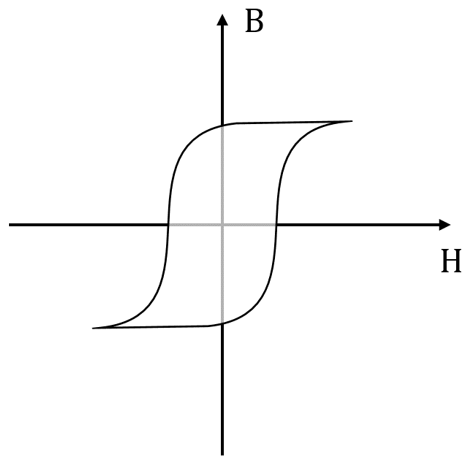
\includegraphics[width=0.40\textwidth]{chap2/images/large_bh_loop.png}
                \label{fig:chapter/background/bh loop/large}
            }
            \qquad
            \subfloat[]{
                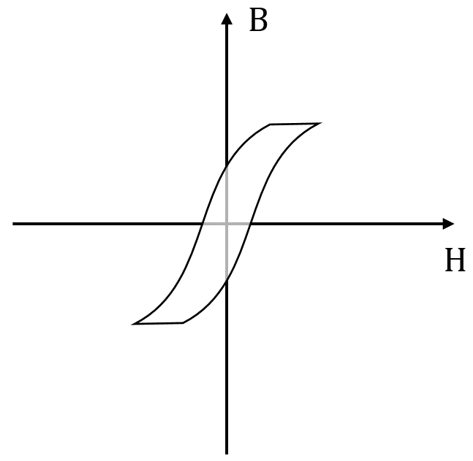
\includegraphics[width=0.4\textwidth]{chap2/images/narrow_bh_loop.png}
                \label{fig:chapter/background/bh loop/narrow}
            }
            \caption{
                Illustration of magnetic hysteresis for different ferromagnetic materials. Large $B-H$ curve (a) retains a significant fraction of magnetic flux density $B$ when the applied magnetic field $H$ is removed. Narrow $B-H$ curve (b) implies small energy dissipated when the applied magnetic field H is changing in the material.
            }   \label{fig:chapter/background/bh loop}
        \end{figure*}
        
        
        The gradient of the $B-H$ curve is the value of material permeability $\mu$. Ferromagnetic material with a linear $B-H$ relationship, or in other words, materials having the constant permeability over a range of applied H-fields, are relatively easier to model because losses caused by the changing of H-field can be predicted without the need of iterative numerical methods. There have been many successes with modelling Neodymium NdFeB rare-earth permanent magnets because this material has high $B_{rem}$, high $H_{ci}$, and $B-H$ linearity over a wide range of applied $H$-field. Iron, however, has a relatively low $B_{rem}$ and narrow range of $B-H$ curve linearity which makes it difficult to predict losses caused by magnetic hysteresis. Although a lookup table can be created, however, such a data table needs to include frequency in addition to the fields amplitude. 
        
        
        A wide hysteresis loop, as illustrated in Figure\,\ref{fig:chapter/background/bh loop/large} may seem ideal for permanent magnets because the material will likely retain a large fraction of magnetization field once the driving field is removed. However, for materials used as a magnetic conductor to close the effective air gap like iron, a narrow hysteresis loop is desired. A narrow hysteresis loop, as shown in Figure\,\ref{fig:chapter/background/bh loop/narrow} implies that only a small amount of energy is lost during repeated shifting of the magnetization which occurs every time the magnet moves relative to the iron. Hysteresis loss is still a tough effect to solve analytically.
        
        
        As mentioned above, in a magnetized ‘hard’ ferromagnetic material such as a permanent magnet, there exists a net magnetic moment without an applied external field $H$. The more convenient representation for a permanent magnet introduces $M_0$ as an additional magnetic moment term:


        \begin{equation}
            B = \mu_0 (H + M + M_0)
            \label{eq:B field equation 1}
        \end{equation}   
        
        \begin{equation}
            B = \mu_0 \mu_r H + \mu_0 M_0
            \label{eq:B field equation 2}
        \end{equation}   
        
        \begin{equation}
            M_0 = \frac{B_{rem}}{\mu_0}
            \label{eq:B rem equation}
        \end{equation}  
        
    
    % -----------------------------------------------------------------------------------
    % --- NEW SUB SECTION --- NEW SUB SECTION --- NEW SUB SECTION --- NEW SUB SECTION --- 
    % -----------------------------------------------------------------------------------
    \subsection{Force production}                   \label{Chapter:background/electromagnetic field theory/force production}
    
        Lorentz's force equation describes force $\overrightarrow{f}$ experienced by a charge $q$ moving with a velocity $\overrightarrow{v}$:
        
        
        \begin{equation}
            \overrightarrow{f} = q(\overrightarrow{E} + \overrightarrow{v} \times \overrightarrow{B})
            \label{eq:lorentz force equation}
        \end{equation}   
        
        
        where there is a electric field $\overrightarrow{E}$ and a magnetic field $\overrightarrow{B}$. The first part of the equation describes the force exerted on a charge by the mere presence of an electric field $\overrightarrow{E}$. The second part of the equation describes the force created when a moving charge is crossing a magnetic field $\overrightarrow{B}$. Force $\overrightarrow{F}$ is the resultant force acting on a body of given volume $V$ with current density $J$ flowing through volume $V$:
        
      
        \begin{equation}
            \overrightarrow{F} = \int_V \overrightarrow{J} \times \overrightarrow{B} \mathrm{d}v
            \label{eq:volume generalized lorentz}
        \end{equation} 
        
        
        Calculating the cross product of the free current density and the magnetic flux density requires knowledge of the total current density in the domain considered, i.e., the sum of all free and microscopic currents at an atomic level.
        Instead, to calculate the electromagnetic force acting on a body, we can perform surface integration of the Maxwell's stress tensor $\mathbb{T}$ around the body enclosed by surface area $S$ and an outward unit normal to the bounding surface $\overrightarrow{n}$:
        
        
        \begin{equation}
            \overrightarrow{F} = \oint_{S} \mathbb{T} \cdot \overrightarrow{n} \mathrm{d}s
            \label{eq:surface generalized lorentz}
        \end{equation}     


        % where the Maxwell's stress tensor, $\sigma$, consists of only the magnetic field component but not the electric field component, is coordinate system independent and defined as:


        % \begin{equation}
        %     \label{eq:maxwell stress tensor}
        %     \sigma_{ij} = \frac{B_i B_j}{\mu_0} - \delta_{ij} \frac{| \overrightarrow{B} |^{2}}{2\mu_0}
        % \end{equation}
                
        % \begin{equation}
        %     \notag
        %     \begin{split}
        %         \text{where Krocher delta} \quad \delta_{ij} =
        %             \begin{cases}
        %                 1       & \text{if $i=j$,}\\
        %                 0       & \text{if otherwise}
        %             \end{cases}
        %     \end{split}
        % \end{equation}
        

% ===================================================================================================
% === NEW SECTION === NEW SECTION === NEW SECTION === NEW SECTION === NEW SECTION === NEW SECTION ===
% ===================================================================================================
\section{Modelling techniques for motors}           \label{Chapter:background/modelling techniques for designing motors}


    Electric machines are devices that either produce force as a product of electric current and magnetic field, or harvest electric current from a conductor in contact with a changing magnetic field. It is necessary to estimate rated power, efficiency, and losses to optimize and achieve design goals. These estimations often require calculation to work out one or more machine characteristics using different forms of Maxwell's equations, governed by the relationship between constitutional materials, geometry, and configurations that apply to individual machines. Quasi-static or low-frequency assumption has been extensively used to model synchronous motors. Methods to solve quasi-static Maxwell's equations indirectly via either magnetic vector potential $A$ or scalar potential $\varphi$ are mentioned in Section\,\ref{Chapter:background/electromagnetic field theory/quasi-static maxwell equations}. The method for solving Maxwell's equations to model electric machines can fall under three categories: numerical, analytical or semi-analytical. Recently, motor types yet to be well understood can be modelled using empirical methods by collecting a vast amount of simulation data and fitting the motor variables and performance onto a set of non-linear equations.


    % -----------------------------------------------------------------------------------
    % --- NEW SUB SECTION --- NEW SUB SECTION --- NEW SUB SECTION --- NEW SUB SECTION --- 
    % -----------------------------------------------------------------------------------
    \subsection{Numerical methods}                  \label{Chapter:background/modelling techniques for designing motors/numerical methods}
    
    
        Mathematically speaking, Maxwell's equations are \acsp{PDE}. Numerical methods approximate the \acsp{PDE} into a system of linear equations by discretization of the spatial domain into smaller building blocks. These components are also called meshes, which are often triangular in the case of two-dimensional and tetrahedral for three-dimensional problems. Fine discretization, at the cost of an increase in computation effort, generally gives better results than coarse discretization. Boundary conditions will alter the set of governing equations appropriately. If discretization occurs throughout the body of the materials, this method is referred to as a \ac{FEM} or \ac{FEA}\,\cite{Boglietti2009EvolutionMachines,Huang2009}. In case the discretization happens only at the surface of the materials, it is referred to as a \ac{BEM}\,\cite{Fetter1998TransientCoil,Qaseer2014HybridMotor}. 
        
        \acs{FEA} is widely used because it can solve complex geometry, include nonlinear material properties and account for coupling between multiple types of physics (thermal, magnetic, mechanical) using nonlinear iterative algorithms\,\cite{Sizov2013AutomatedEvolution}. Out of the three categories, the numerical method requires the most computation effort. Often, \acs{FEA} requires too much computational effort to be used directly in optimization. Tuning for a single parameter may take several hours or days, depending on the mesh density. \acs{FEA} is usually used to evaluate the accuracy of analytical and semi-analytical models.

    
    % -----------------------------------------------------------------------------------
    % --- NEW SUB SECTION --- NEW SUB SECTION --- NEW SUB SECTION --- NEW SUB SECTION --- 
    % -----------------------------------------------------------------------------------
    \subsection{Analytical methods}                 \label{Chapter:background/modelling techniques for designing motors/analytical methods}
    
    
        The most commonly used analytical modeling method is known as \ac{MEC}. Similar to \acs{FEA}, the geometry is discretized. However, the number of elements is much smaller. Prior knowledge of flux distribution is necessary to construct an accurate model. Discretized flux tubes with assumed constant flux distribution are used to simplify the real problem. Instead of finding a direct solution for the Maxwell's equations, the flux distribution represented in terms of lumped flux tubes is modelled using electric circuit analogy. Magnetic flux is obtained as a product of given \ac{MMF} due to the magnetic field source.  
        
        
        \acs{MEC} takes a simple form and very low computational time. Saturation can be taken into account by splitting a soft magnetic object into multiple flux tubes with permanence dependent upon the magnetic field strength through each tube. Effects such as flux leakage and fringing are difficult to take into account because this approach assumes flux enters and leaves solely in the axial direction of the flux tubes. The differences in relative permeability between the regions are usually not taken into account, and relative permeability for air is assumed as unity. For the stated reasons, \acs{MEC} performs poorly in structures with large air gaps or structures with no magnetic bridge (iron) at all\,\cite{DeBoeij2006}. 
        
        
        The exact analytical approach to modelling electromagnetic environment in the literature has obtained success with modelling the magnetic fields of permanent magnet\,\cite{Ravaud2010}. Other analytical methods include solving complex functions and Schwarz–Christoffel transformation\,\cite{Zarko2006}, and motor phase circuit modelling\,\cite{Proca2003}.
        
        
    % -----------------------------------------------------------------------------------
    % --- NEW SUB SECTION --- NEW SUB SECTION --- NEW SUB SECTION --- NEW SUB SECTION --- 
    % -----------------------------------------------------------------------------------
    \subsection{Semi-analytical methods}            \label{Chapter:background/modelling techniques for designing motors/semi-analytical methods}
    
    
        One of the most popular semi-analytical methods takes the form of \ac{HM}. This approach uses the harmonic series or Fourier series to express the magnetic field formulation in 2D and 3D, based on the theory of transfer relation\,\cite{Melcher1981}. The problem is divided into material regions whose boundaries are orthogonal with axes of the coordinate system. The magnetic potentials in the quasi-Halbach magnet array and poly phase winding can be described in terms of a Fourier series. In each region, the equations for vector or scalar magnetic potential can take the form of Laplace or Poisson equations in Cartesian coordinates\,\cite{Trumper1993,Wang1999}. In cylindrical coordinates, the equation for magnetic potential takes the form of the Bessel function\cite{Gysen2008,Ruddy2011a,Gysen2011a}. The most widely used method to solve for the magnetic potential is separation of variables method. The coefficients in magnetic flux density equations, made up of magnetic potential terms are obtained by applying the boundary equations. The magnetic field can then simply be found via the constitutive relationship with magnetic flux density.
        
        
        This modelling technique is excellent for periodic geometry as in long stroke linear machines. Since long stroke synchronous motors have repeating segments of the same structure, the analysis only needs to be limited to a single wavelength with periodic boundary conditions. The end effect is dealt with separately. \acs{HM} is capable of taking linear material properties into account although iron is often assumed to be infinitely permeable. Models which can account for saturation exist in form or diffusion equation or adopt an iterative method that calculates the magnetic field based on the nonlinear B-H curve. \acs{HM} can compute slower than \acs{MEC} but faster than \acs{FEM}. High accuracy and relatively good speed allow HM approaches to be used directly in multi-variable optimization. Different motor geometry configuration requires a different set of \acsp{PDE} to be solved in order to determine the general solution for the magnetic potential in each spatial region. This is a mathematically rigorous process. In validating solutions to the \acsp{PDE}, the tests are checking for continuity behaviour of underlying magnetic fields, and strong agreement with \acs{FEM} results.
        
        
        \ac{MCM} is an alternative method resulting from the use of Green’s integrals to solve Maxwell's equations. Volume integrals are used to obtain magnetic scalar potential under the assumption that the materials used are current free. It is not possible to model the magnetic field due to current using the scalar potential, and thus reduced scalar potential\,\cite{Gong2009} is introduced for this purpose. The reduced scalar potential is robust and convenient for calculating eddy loss in soft ferromagnetic materials\,\cite{Xu2004,Bowler1987,Rubinacci2004}. Magnetization in permanent magnets is replaced by equivalent surface and volume magnetic charge terms with unit permeability. Only constant permeability on the whole domain is considered. \acs{MCM} has not achieved the level of accuracy that \acs{HM} has.
        
    
    % -----------------------------------------------------------------------------------
    % --- NEW SUB SECTION --- NEW SUB SECTION --- NEW SUB SECTION --- NEW SUB SECTION --- 
    % -----------------------------------------------------------------------------------
    \subsection{Empirical methods}                  \label{Chapter:background/modelling techniques for designing motors/empirical methods}


        Due to the complex flux path in motor typologies such as Flux Switching Motors and Transverse Flux Motors, reflected by the difficulty in semi-analytical modelling for this type of motor, the literature typically makes use of $\mathrm{2D}$ or $\mathrm{3D}$ \acs{FEA} to accurately predict the thrust and cogging force. Traditionally, during the optimization process, each performance valuation requires one FEM evaluation. This means the simulation is only needed once. Thus, this approach is considered having poor data re-use, and unpredictable optimization wait time. Instead, we can approach motor design with the \acf{RSM}, by describing the motor performance metrics using empirical equations\,\cite{Hong2008,Lei2013}, or using an artificial neural network\,\cite{Hadjout2006,Ashabani2010}. Once an arithmetic model is fitted to represent the data set, model inference time is a number of magnitudes lower than the simulation time for each valuation. A high number of recent motor design and control research has obtained various degree of success with this approach\,\cite{Hwang2007,Lee2012,Kim2006,Jung2015,Hong2018}. 
        
        
        In a high order \acs{RSM} problem with many input variables, high sampling levels for each input are the key to obtaining accurate model predictions. However, the time and computation effort required are growing exponentially with each additional parameter and sampling level for existing parameter. Planning and execution of \acs{RSM} is in this sense a data exploratory exercise. It is difficult to predict what range of data is needed ahead of time.


% ===================================================================================================
% === NEW SECTION === NEW SECTION === NEW SECTION === NEW SECTION === NEW SECTION === NEW SECTION ===
% ===================================================================================================
\section{Optimization methods}                      \label{Chapter:background/optimization methods}
    
    
    Mathematical optimization techniques offer a methodical way of approaching design problems. Optimization is commonly performed by minimizing cost functions and can be applied to a wide variety of applications:
    
        
    \begin{equation}
        \begin{array}{rll}
            \textbf{minimize}       & \small{objective\,\,function}         & f(x)\\ 
            \textbf{subject to}     & \small{inequality\,\,constraints}     & g_i(x) \leqslant 0, \text{for } i= 1,...,m,\\ 
                                    & \small{equality\,\,constraints}       & h_i(x) = 0, \text{for } j= 1,...,n,\\ 
                                    & \small{variable\,\,space}             & x \in X
        \end{array}
    \end{equation}
    
    
    An alternative is the direct grid search or exhaustive search, in many cases attempt to consider the complete design space. By mapping the performance of every single machine design in a discretized variables to a performance index value, this method can help identify a Pareto front of designs in which the performance could not be further improved. The most suitable machine can then be selected from the group of Pareto-optimum designs, based on the specific requirements and trade-offs of the application.
    
    
    % -----------------------------------------------------------------------------------
    % --- NEW SUB SECTION --- NEW SUB SECTION --- NEW SUB SECTION --- NEW SUB SECTION --- 
    % -----------------------------------------------------------------------------------
    \subsection{Optimization problem classification}    \label{Chapter:background/optimization methods/optimization prob classification}

        
        Some problems only allow variables to take on discrete values, often a subset of integers, whereas other variables can be any real values. Therefore, optimization problems can be classified based on the nature of the variables:

        \begin{itemize}
            \item Discrete optimization - all variables take the form of discrete or boolean values,
            \item Continuous optimization - all variables are continuous
            \item Mixed-integer optimization - some variables in the are discrete while others take continuous values
        \end{itemize}
   
        Another distinction to have is whether the problem is constrained or not. The constraint may be as simple as being bound to the input variable of the objective function to be minimized, or more complex like explicit equal or greater than equal relationships among the variables. Unconstrained optimization problems arise directly from a limited set of applications. In the case of motor design, there often exist limitations such as a desired weight or length or tolerable cogging force.
        
        
        Most optimization problems will have a single objective function to be minimized. However, there are multi-objective problems where people are more interested in the trade-off between the objectives function instead of finding a single satisfactory design. For instance, the problem requires the lightest motor while maximizing force output. In practice, multi-objective problems with multiple objectives will be rearranged as a single objective problem by replacing some objectives as constraints, or by creating a new objective function such as a weighted combination of the original objective functions.
        

    % -----------------------------------------------------------------------------------
    % --- NEW SUB SECTION --- NEW SUB SECTION --- NEW SUB SECTION --- NEW SUB SECTION --- 
    % -----------------------------------------------------------------------------------
    \subsection{Optimization in motor design}        \label{Chapter:background/optimization methods/optimization in motor design}
    
    
        The increase in speed and reduction in price of computer hardware, together with the development of faster algorithms as well as highly accurate \acs{FEA} models allow theoretical optimum design to be obtained. The design of permanent magnet motors or actuators has been discussed in many textbooks; however, a standard method does not exist since the application together with different sets of applicable constraints determines the strategy. The design of \acsp{PMLSM} for \acs{NFJI} is no exception. Ideally, the actuator should have high force density and the energy losses should be minimal. 
    
        
        One class of optimization methods is a group of gradient methods, in which the search direction is determined by the local gradient of the objective function at the current search point. Such algorithms are referred to as non-linear programming. Though straight forward to implement, these algorithms tends to converge to local optimum. If the problem at hand is a mixed integer optimization problem, the discrete variables will be treated separately by considering all possible combinations of the discrete variables as separate optimization problems\,\cite{Ruddy2015a}. This class of optimization algorithm has been demonstrated to be working well with semi-analytical and analytical modeling techniques\,\cite{Overboom2010,Aleksandrov2018,Fang2008}. 
        
        
        The other class of optimization algorithm is evolutionary methods. They are probability based algorithms which start with an initial population of design candidates and simulate a breeding environment. The characteristics of each design are used to generate a fitness value to indicate its level of performance with respect to other designs in the population. After each generation, breeding is carried out to combine the characteristics of selected parent designs with the hope of yielding a better next generation of designs. This class of algorithm has the capacity to handle both discrete and continuous variables. The random mutation guarantees to some extent that we see a wide range of solutions. However, it is rather tricky to choose parameters such as the number of generation, the population and the mutation probability. Despite the experiment-like nature of this class of methods, the literature has applied this method extensively in motor design, starting from proven analytical and semi-analytical models\,\cite{Isfahani2007,Li2014,Mallik2017,RuiHuang2008}.
        
        
        Direct use of \acs{FEM} is far less suitable for optimization purposes due to the long computation time taken to evaluate a single objective function. Even with simple structures, the creation of mesh can be the most time-consuming task. One way to overcome this limitation is to replace the online \acs{FEM} function evaluation with a simplified function that requires far less time to compute. As mentioned in Section\,\ref{Chapter:background/modelling techniques for designing motors/empirical methods}, these methods are classified as empirical modelling methods. Once there exists a simplified model to represent the design space, gradients and evolutionary methods can be applied to find the globally optimal motor design\,\cite{Ashabani2010,Lee2012,Giurgea2007,Hasanien2010, Hasanien2011,Zhang2017}. 
